% !TEX root = ../relatorio.tex

\subsection{Arquitetura de DSP}

A fim cumprir os objetivos listados acima, proponho a arquitetura descrita na figura \ref{fig:arquitetura}.

A aplicação processará sequencialmente as amostras de entrada e aplicará um filtro simplificado calculado a partir de 10 filtros passa-faixa dividindo o espectro entre as frequências requeridas no projeto. Para o cálculo dos valores do gráfico de barras, aplicaremos periodicamente uma FFT, somando as energias das faixas especificadas.

\begin{figure}[h]
    \centering
    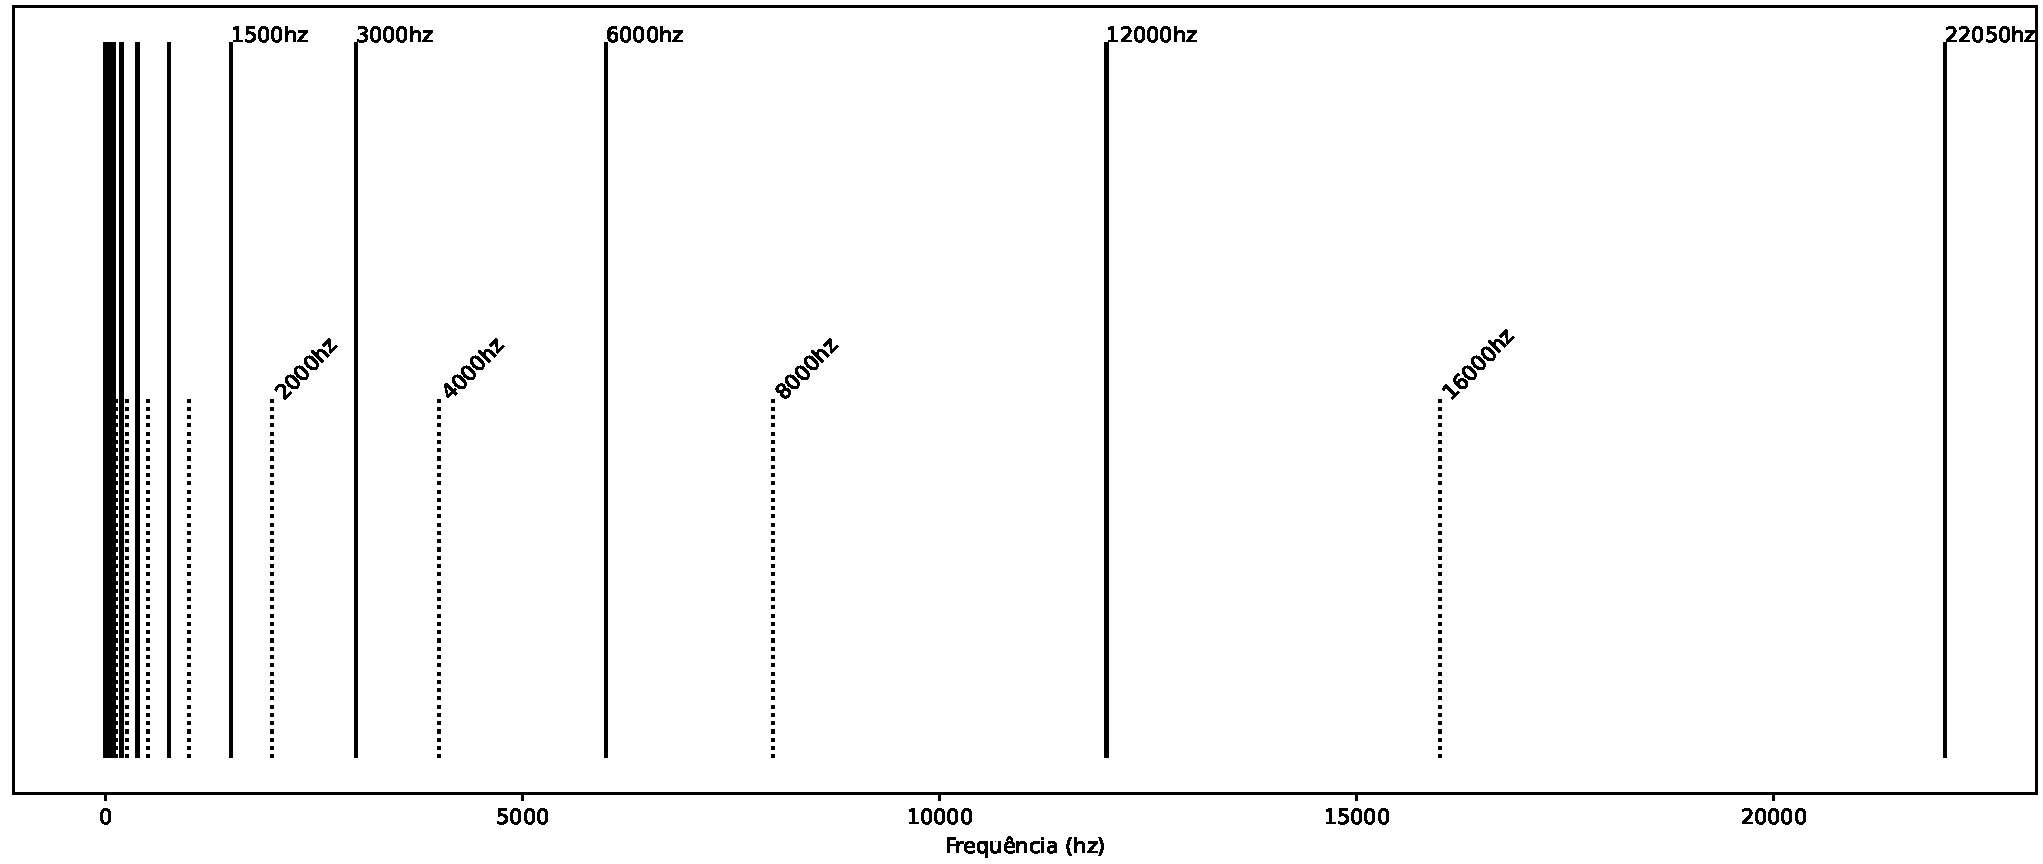
\includegraphics[scale=.45]{fig/Bands.pdf}\\
    \small{Pontilhadas: frequências "centrais" das bandas}\\
    \small{Sólidas: frequências-limite das bandas}
    \caption{Bandas de filtragem}
    \label{fig:bandas}
\end{figure}


\subsection{Detalhes e justificativa de implementação}


Inicialmente propus a arquitetura ilustrada na figura \ref{fig:arquiteturar}, que consistia em aplicar separadamente os 10 filtros e guardar seus resultados em acumuladores para calcular a energia de cada banda.

Mesmo tendo uma complexidade maior que a FFT, intuitivamente imaginei que para a pequena quantidade de filtros que temos e para uma largura reduzida de filtro, este método poderia custar menos operações.

\begin{figure}[h]
    \centering
    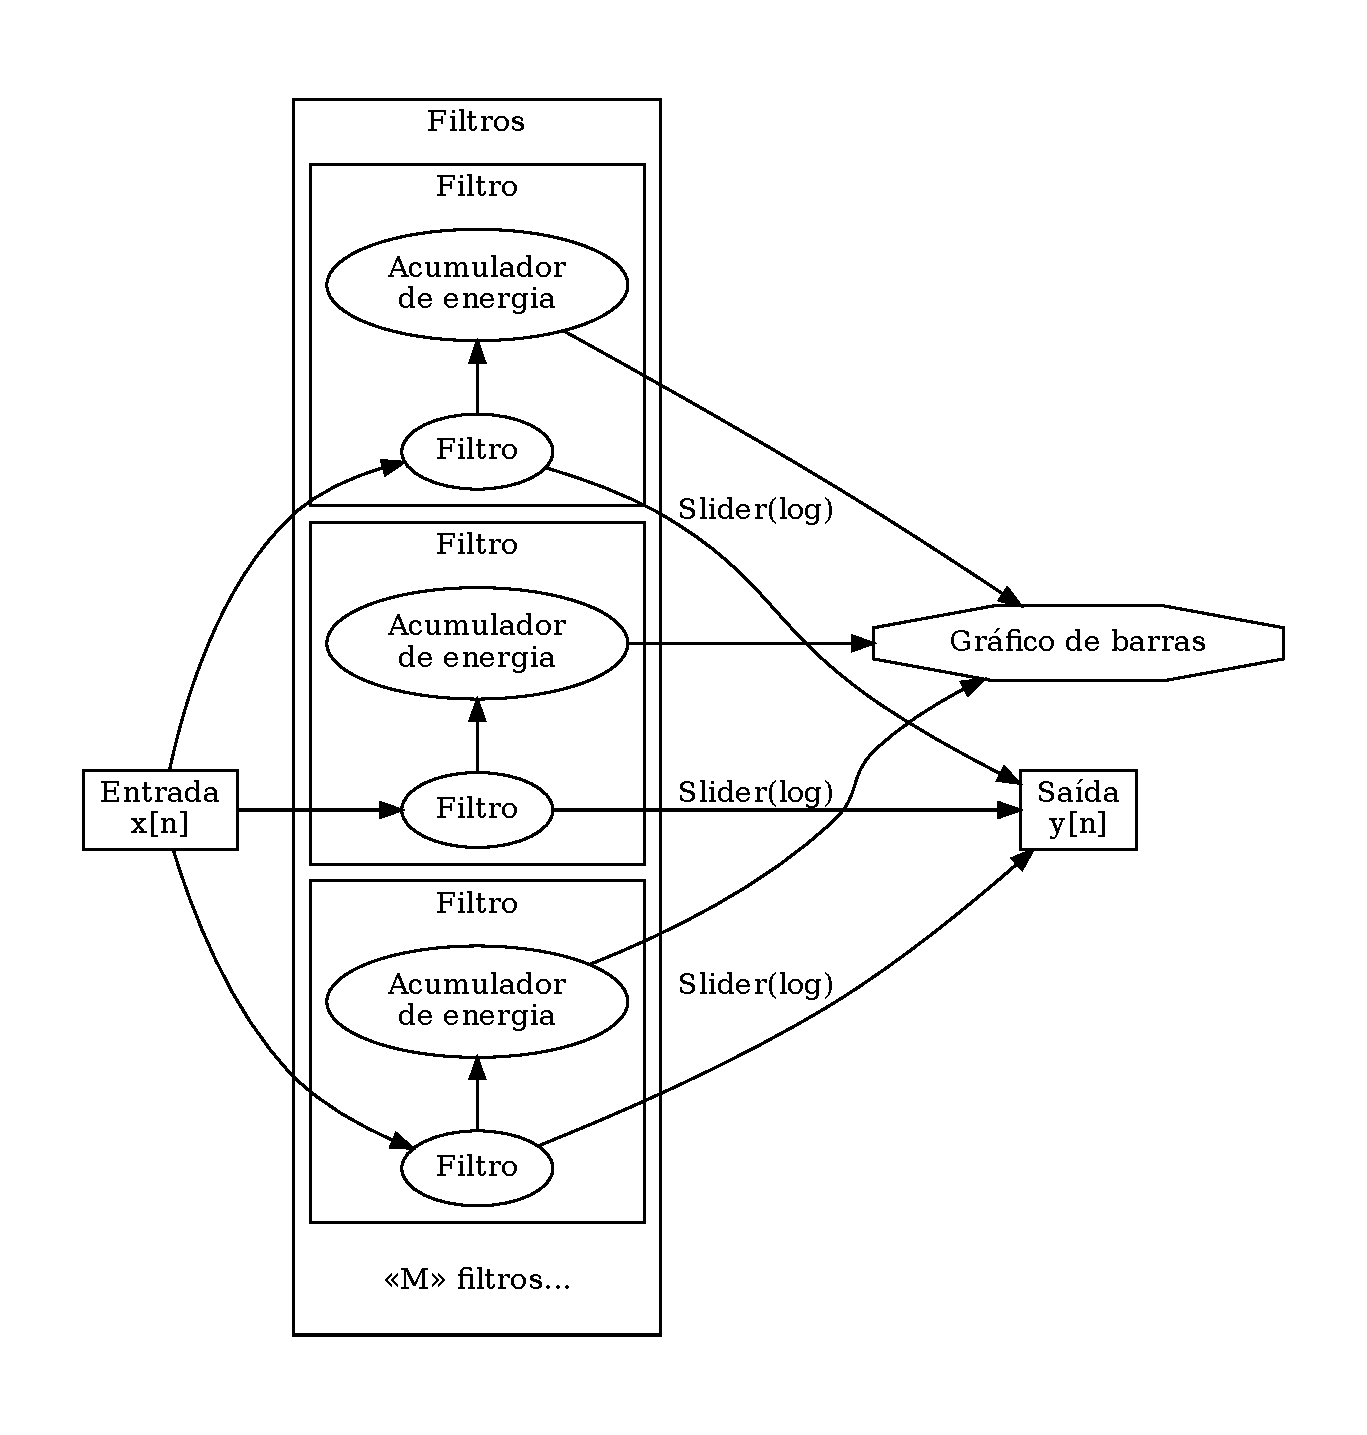
\includegraphics[scale=0.5]{fig/arquitetura.pdf}
    \caption{Má arquitetura proposta}
    \label{fig:arquiteturar}
\end{figure}

\break

Buscando uma comparação mais concreta entre essa proposta e a da figura \ref{fig:arquitetura}, fiz uma análise mais detalhada.

\begin{figure}[h]
    \centering
    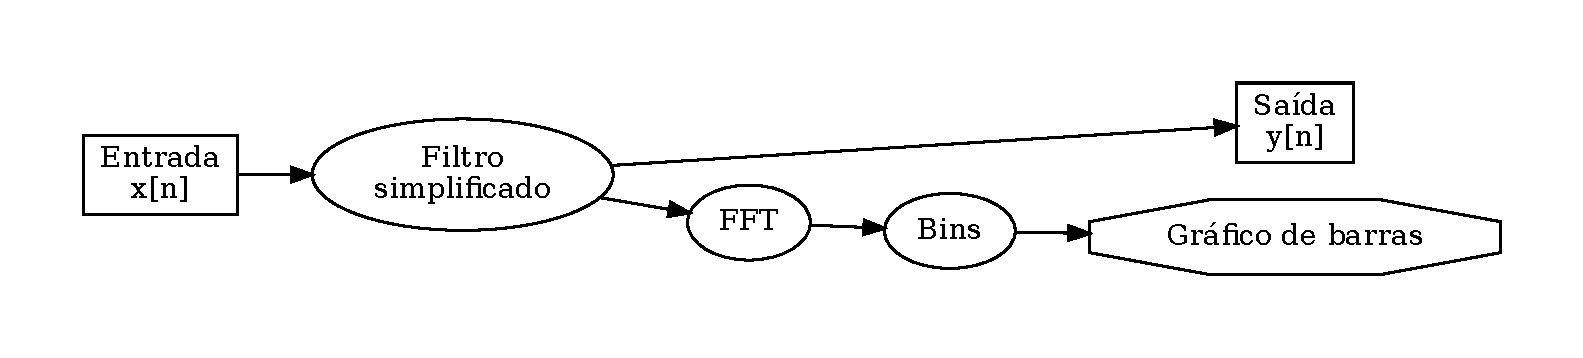
\includegraphics[scale=0.5]{fig/arquiteturafft.pdf}
    \caption{Nova arquitetura proposta}
    \label{fig:arquitetura}
\end{figure}

Na arquitetura sem FFT, para uma quantidade de amostras $S$ e $M$ filtros FIR de largura $W$, o número de operações a serem feitas para calcular todos os valores necessários será:

\begin{itemize}
    \item Multiplicações: $S(WM)$
    \begin{itemize}
        \item $WM$ para multiplicação das amostras pelos coeficientes em ($\sum\limits_i^W a_ix[n-i]$) e ponderação dos sliders;\\
        (Para um peso $w$, $w\sum\limits_i^W a_ix[n-i]=\sum\limits_i^W (a_iw)x[n-i]$, então pré-calculamos $a_iw$)
    \end{itemize}
    \item Somas/Subtrações: $S(WM+M+2M)$
    \begin{itemize}
        \item $WM+M$ para os filtros:
        \begin{itemize}
            \item $WM$ para o somatório $\sum\limits_i^W a_ix[n-i]$;
            \item $M$ para somar todos.
        \end{itemize}
        \item $2M$ para o acumulador de energia:
        \begin{itemize}
            \item 1 soma para adicionar a amostra atual;
            \item 1 subtração para remover a última amostra.
        \end{itemize}
    \end{itemize}
\end{itemize}

Para a arquitetura com FFT, teríamos, presumindo $S=2^p$ e um número de amostragens do gráfico de energia ao longo do \textit{chunk} de memória $G=2^k,k<p$, gerando "pacotes" de $L=S/G$:

\begin{itemize}
    \item Multiplicações: $S(W) + G\frac{L}{2}log_2L$
    \begin{itemize}
        \item $W$ para multiplicação das amostras pelos coeficientes;
        \item $\frac{L}{2}log_2L$ para a FFT.
    \end{itemize}
    \item Somas/subtrações: $S(W)+G(Llog_2L+L)$
    \begin{itemize}
        \item $W$ para o somatório de $y[n]$.
        \item $Llog_2L$ para a FFT;
        \item $L$ para aglomeração das "bins" da FFT.
    \end{itemize}
\end{itemize}

Presumindo 4096 amostras, podemos explorar as complexidades das duas implementações para diversas combinações dos parâmetros $W$ e $G$.

Para \textbf{todas} as combinações exploradas (todos W entre 1 e 500, todos G entre 1 e 11), o método com FFT foi superior (vide \texttt{misc/operacoes.py}).

\begin{table}[h!]
    \begin{center}
        \begin{tabular}{ |c|c|c| }
        \hline
         $N_{fft}/N_{naive}$ & \textbf{Multiplicações} & \textbf{Somas} \\ 
        \hline
        Média & 9.68 & 9.64 \\  
        Máxima & 9.98 & 10 \\
        Mínima & 1.53 & 3.07 \\
        \hline
        \end{tabular}
        \caption{Razão entre o número de operações da abordagem com FFT e sem ($N_{fft}/N_{naive}$)}
    \end{center}
\end{table}

\subsection{Arquitetura da aplicação}

A aplicação se dividirá em três componentes principais:

\begin{itemize}
    \item Provedor de informação dos sliders;
    \begin{itemize}
        \item Codificado em Python;
        \item Apresentará a interface de alteração dos filtros para o usuário;
        \item Proverá os coeficientes do filtro para o processador de sinais via socket UNIX.
    \end{itemize}
    \item Host de filtragem;
    \begin{itemize}
        \item Codificado em C;
        \item Receberá coeficientes de filtragem via socket UNIX;
        \item Receberá um feed de som do PulseAudio, aplicará o filtro FIR caracterizado pelos parâmetros guardados e enviará um feed de som de volta ao PulseAudio;
    \end{itemize}
    \item Visualizador de gráfico de barras.
    \begin{itemize}
        \item Codificado em Python;
        \item Receberá um feed de som do PulseAudio e gerará um gráfico de barras de intensidade de cada banda.
    \end{itemize}
\end{itemize}

\begin{figure}[H]
    \centering
    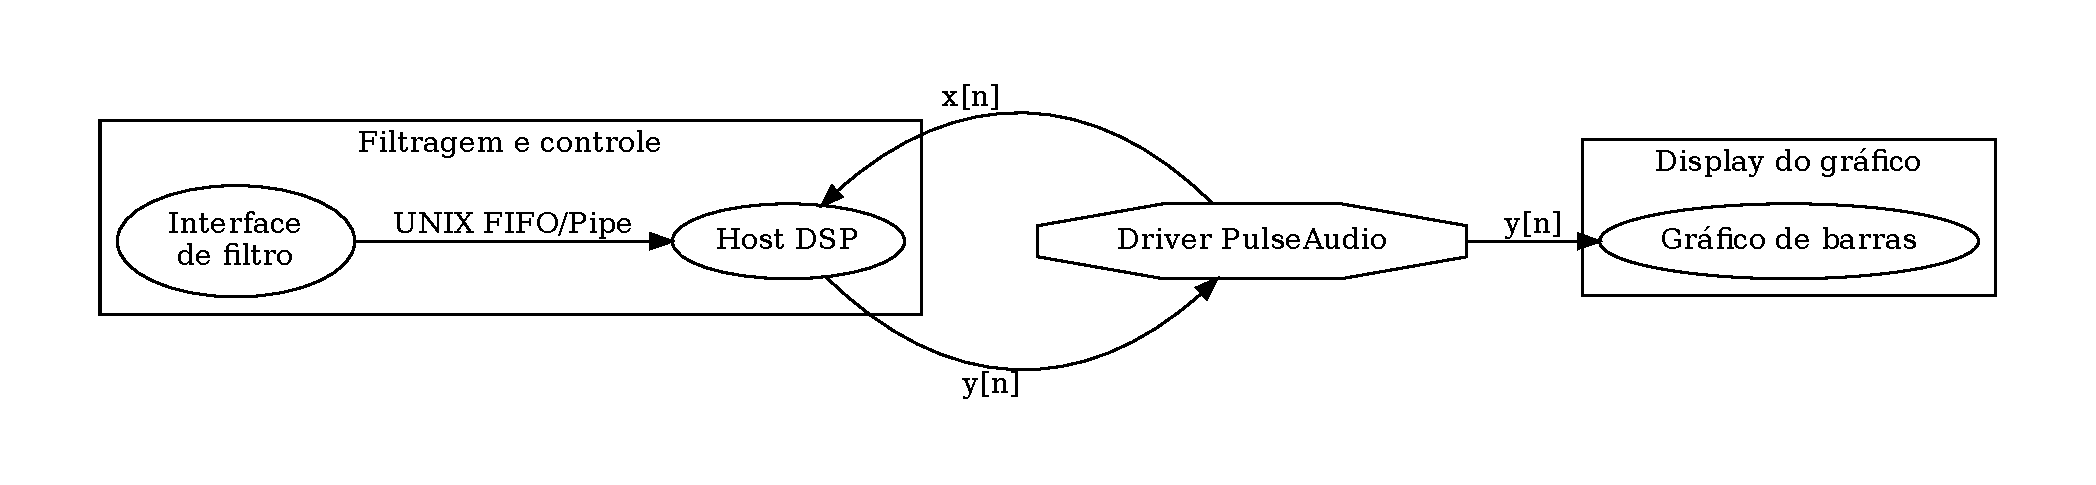
\includegraphics[scale=0.45]{fig/app.pdf}
    \caption{Processos e conexões relevantes}
    \label{fig:app}
\end{figure}

Destes processos, dois grupos são basicamente independentes:

\begin{itemize}
    \item Processos de controle e filtragem
    \begin{itemize}
        \item Lidam com a filtragem do áudio e configuração do filtro;
        \item Lidam com a interação com o usuário.
    \end{itemize}
    \item Processo de display do gráfico
    \begin{itemize}
        \item Lida com o cálculo das intensidades de cada \textit{bin} de frequências.
        \item Lida com a ilustração das intensidades com um gráfico de barras.
    \end{itemize}
\end{itemize}

O isolamento dos dois grupos, bem como o desenho do host de DSP de forma "reativa" (funciona continuamente até que alguma alteração venha da interface, com mínima interrupção) permite que o feed de som seja contínuo, sem falhas provindas de gargalos de processamento, e que o display visual, para o qual continuidade não é tão importante, possa lidar com o feed de som em seu próprio "ritmo".

\break